\documentclass[a4paper,oneside]{article}
\usepackage[utf8]{inputenc}
\usepackage[spanish]{babel}
\usepackage[margin=1in]{geometry}
\usepackage{amsmath}
\usepackage{amsfonts}
\usepackage{amssymb}
\usepackage{enumitem}
\usepackage{hyperref} 
\usepackage{graphicx}
\usepackage{url}
\usepackage{breakurl}
\hypersetup{pdftex,colorlinks=true,allcolors=black}
\hypersetup{
    pdftitle={},
    pdfauthor={Pablo Riutort Grande},
    pdfsubject={},
    bookmarksnumbered=true,     
    bookmarksopen=true,         
    bookmarksopenlevel=1,       
    colorlinks=true,            
    pdfstartview=Fit,           
    pdfpagemode=UseOutlines    % this is the option you were lookin for
}
\usepackage{listings}
\usepackage{xcolor}
\usepackage{hypcap}
\usepackage{caption}
\definecolor{codegreen}{rgb}{0,0.6,0}
\definecolor{codegray}{rgb}{0.5,0.5,0.5}
\definecolor{codepurple}{rgb}{0.58,0,0.82}
\definecolor{backcolour}{rgb}{0.95,0.95,0.92}
\lstdefinestyle{mystyle}{
    backgroundcolor=\color{backcolour},   
    commentstyle=\color{codegreen},
    keywordstyle=\color{magenta},
    numberstyle=\tiny\color{codegray},
    stringstyle=\color{codepurple},
    basicstyle=\ttfamily\footnotesize,
    breakatwhitespace=false,         
    breaklines=true,                 
    captionpos=b,                    
    keepspaces=true,                 
    numbers=left,                    
    numbersep=5pt,                  
    showspaces=false,                
    showstringspaces=false,
    showtabs=false,                  
    tabsize=2
}
\lstset{style=mystyle}
\usepackage{xparse}
\usepackage{comment}
\NewDocumentCommand{\codeword}{v}{%
\texttt{{#1}}
}
\author{Pablo Riutort Grande}
\title{
	Seguridad del software\\
	\vspace{1cm}
	\textbf{Práctica}
	\vspace{1cm}\\UOC - MISTIC
}

\begin{document}
\maketitle
\pagebreak
\tableofcontents
\lstlistoflistings
\listoffigures

\pagebreak

\begin{comment}

La realización de la práctica consta de tres partes
Creación de un programa con código vulnerable
Creación de un shellcode para el código vulnerable del programa creado
Aplicar Reverse Engineering o PenTesting
Esta práctica se puede realizar en un entorno Windows, Linux o Android (o emulador Android).
Se trata de realizar un programa sencillo con un código que sea vulnerable y crear un shellcode para este código. No se debe realizar ni un gran programa ni un programa complicado porque este no es el objetivo de la asignatura. Lo que se pretende es crear un shellcode que logre ejecutarse tras aprovechar un exploit en una aplicación.
Debéis realizar vosotros mismos el programa y el shellcode. Podéis elegir el tipo de vulnerabilidad, por ejemplo: Integer overflow, Desbordamiento de pila Stack overflow o Desbordamiento de heap.
Aplicar Reverse Engineering o PenTesting : En esta práctica debéis aplicar Reverse Engineering o PenTesting. En el caso del Reverse Enginnering, aunque el programa lo habéis realizado vosotros mismos, debéis analizar con técnicas de Reverse Enginnering cómo y por qué el programa es vulnerable y cómo acuta el Shellcode. En el caso de elegir Pentesting, debéis realizar un test de penetración detectando la vulnerabilidad y la actuación del shellcode.
 Memoria
Documento en formato PDF con la siguiente estructura básica, también podéis agregar los apartados o anexos que creáis convenientes:

 Descripción de la vulnerabilidad que habéis creado y del shelcode así como el desarrollo del Reverse Engineering o el Pentesting
 
Entorno de desarrollo: Windows o Linux, versión del sistema operativo y relación y versiones de todo software utilizado.

Código fuente completo tanto del programa con código vulnerable como del shelcode. El código fuente se debe documentar exhaustivamente.

Análisis: Razonamiento y explicación detallada del funcionamiento del programa vulnerable y del shelcode, paso a paso de la ejecución de los programas, con ejemplos de los valores para los cuales es vulnerable y en los que no es vulnerable, así como de los diversos valores relevantes que tengan en diferentes momentos la pila, los registros y la memoria.

Se deben incluir todas las impresiones de pantalla que sean necesarias para razonar y explicar paso a paso la vulnerabilidad y el shellcode en tiempo de ejecución, con impresiones de pantalla del programa IDA, Immunity, OllyDbg, GDB o el que hayáis elegido, los resultados o valores que aparecen en la consola y otros programas que utilicéis en la realización de la práctica.
Informe de la descripción del problema que tiene el programa y qué solución debería aplicarse para que el programa no fuera vulnerable. (La extensión de este apartado no es necesario que supere la media página)
 Presentación de la práctica
 Fichero ZIP que debe incluir los archivos siguientes:
 Memoria en formato PDF (con el nombre Apellidos_Nombre.pdf )
 Los archivos del código fuente de los programas.
Los archivos ejecutables de los programas.
Otros ficheros que utilicéis en la elaboración de la práctica
Comprobad que los archivos se extraen del fichero ZIP de forma correcta antes de entregar la práctica
\end{comment}

\section{Introducción}
Se aprovechará la vulnerabilidad del stack overflow. Esta vulnerabilidad de la familia del buffer overflow que consiste en mandar datos a un programa que utiliza un buffer no lo bastante grande para almacenarlos. El resultado es que la pila de llamadas (\textit{call stack}) será sobreescrita incluido el puntero de retorno de la función (\textit{Instruction Pointer} o IP). Los datos introducidos sobreescriben el valor del puntero de tal forma que cuando la función ejecuta las instrucciones de retorno transfiere el control al código malicioso introducido por el atacante \cite{buffer}.\\

El entorno de ejecución se trata de una máquina de virtual con Kali Linux de 32 bits: kali-linux-2020.3-live-i386. El programa se ha desarrollado en lenguage C, compilado con gcc versión 9.3.0 y el reverse engineering se ha llevado a cabo mediante el debugger GNU gdb (Debian 10.1-1.5).\\

Para realizar este programa de forma satisfactoria se ha deshabilitado la aleatorización del espacio de memoria o ASLR con el siguiente comando:
\begin{lstlisting}[language=bash]
sysctl kernel.randomize_va_space=0
\end{lstlisting}
El ASLR puede localizar el heap y el stack en posiciones aleatorias de memoria lo que dificulta la predicción la dirección de memoria de la siguiente instrucción \cite{aslr}.\\

Para poder realizar correctamente este ejercicio se debe añadir el argumento --no-pie en la compilación del programa vulnerable. Este flag obliga a gcc a no crear un ejecutable con posición independiente (PIE) que es una precondición para el ASLR \cite{pie}.

\subsection{Programa vulnerable}
El programa desarrollado para esta práctica consiste en sencillamente copiar el contenido de un string dado por puntero a un buffer delimitado [Ver \ref{lst:stack}]. Esta copia se efectuará mediante la función vulnerable $strcpy()$ \cite{strcpy}.\\

Primero importaremos las librerías stdio.h para trabajar con funciones de input/output y string.h para manipular arrays de caracteres o strings.
\lstinputlisting[
	language=C, 
	caption={[stack.c]{Programa de stack overflow}},
	lastline=3
]{stack.c}

A conitnuación se define el método $main()$ que pasará su segundo argumento a la función $copy()$. Es en este argumento donde se hará el ataque puesto que será la sentencia inmediatamente después a la llamada del ejecutable por terminal.

\lstinputlisting[
	language=C, 
	caption={[stack.c]{Programa de stack overflow}},
	firstline=5,
	lastline=7
]{stack.c}

La función $copy()$ únicamente declara un buffer de tamaño fijo y llama a la función vulnerable strcpy donde copia el string dado por parámetro al puntero del array destino, es decir, el buffer.

\lstinputlisting[
	language=C, 
	caption={[stack.c]{Programa de stack overflow}},
	firstline=9,
	lastline=12
]{stack.c}
\newpage

\subsection{Shellcode}
Un shellcode es un conjunto de instrucciones inyectadas y luego ejecutadas por un programa vulnerable. Se utiliza para manipular directamente los registros y la funcionalidad del programa vulnerable. Típicamente se utiliza para llamar a una shell desde la máquina comprometida, de ahí el nombre ``shellcode'' \cite{shellcode}.\\
Para nuestro caso, utilizaremos una llamada al intérprete de comandos Debian Almquist Shell (dash) que suele venir instalada por defecto en las máquinas Debian y se ejecuta al llamar a la instrucción $/bin/sh$ [Fig. \ref{fig:dash}].

\begin{figure}[h!]
  \centering
  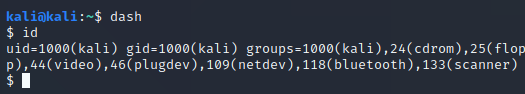
\includegraphics[scale=0.7]{images/dash.png}\\
  \caption{Llamada al intérprete dash desde terminal}
  \label{fig:dash}
\end{figure}

El código que contenga el shellcode puede ser cualquier cosa excepto bytes nulos ya que eso es interpretado como el fin de un string. Para hacer una llamada a la shell en cuestión deberemos inyectar los valores en hexadecimal que codifiquen una llamada a $/bin/sh$ y además inundaremos la memoria con la instrucción NOP que sencillamente es ignorada y pasa a ejecutar la siguiente, creando una reacción en cadena que nos permitirá ejecutar el shellcode. Después, tan solo tendremos que modificar el \textit{Instruction Pointer} de tal forma que la siguiente instrucción a ejecutar caiga en una zona de memoria que contenga una instrucción NOP.\\

Dado que el shellcode se hace manipulando la entrada de datos del programa vulnerable, se ha realizado un script de Python que inyecta el mismo [Ver \ref{lst:shellcode}]. Este programa creará una entrada de texto que inundará la memoria de caracteres NOP e introducirá el código de la llamada a la shell.

\section{Reverse engineering}
\begin{comment}
Aquí es casi paso por paso lo de la web
\end{comment}
Para llevar a cabo el reverse engineering primero ejecutaremos el programa con diferentes entradas para entender el funcionamiento y sus límites. Veremos que la ejecución con demasiados inputs genera un Segmentation Fault que puede ser interesante explotar [Fig. \ref{fig:test1}] [Fig. \ref{fig:test2}].

\begin{figure}[h!]
  \centering
  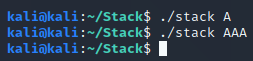
\includegraphics[scale=0.7]{images/test.png}\\
  \caption{Llamada al programa con diferentes parámetros}
  \label{fig:test1}
\end{figure}

\begin{figure}[h!]
  \centering
  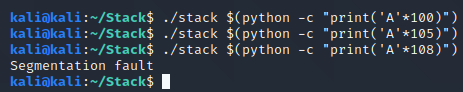
\includegraphics[scale=0.7]{images/test2.png}\\
  \caption{Llamada al programa con parámetros que provocan Segmentation Fault}
  \label{fig:test2}
\end{figure}

Vistas las limitiaciones del programa, podemos pasar a analizar una ejecución normal con gdb y darnos cuenta de que existe la función vulnerable strcpy que es la que provoca el error [Fig. \ref{fig:test3}].

\begin{figure}[h!]
  \centering
  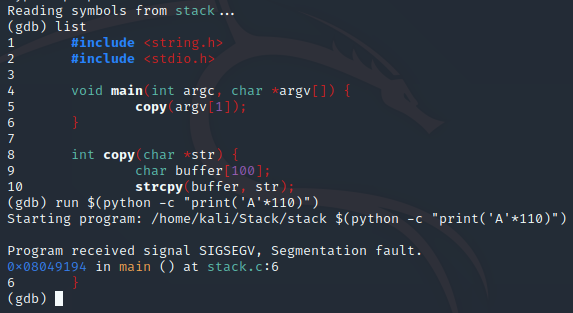
\includegraphics[scale=0.7]{images/test3.png}\\
  \caption{Debugging del programa: Detalle de \textit{Segmentation Fault}}
  \label{fig:test3}
\end{figure}

Podemos ver el contenido de la pila con gdb, recordemos que el registro \$esp indica el top de la pila, entonces podemos leer el contenido de la pila con la instrucción x\textbackslash40x \$esp que nos dará los 40 words siguientes a partir de la dirección correspondiente al registro \$esp.\\
Dada una entrada lo suficientemente grande podemos ver el contenido de la pila inundado [Fig. \ref{fig:stack_content}]. De hecho, si la entrada es lo suficientemente grande podemos llegar a sobreescribir la dirección del fondo de la pila (\$esp), es decir, la dirección de retorno de la función, en nuestro caso 0xbffff168 [Fig. \ref{fig:registers}] [Fig. \ref{fig:overflow}] [Fig. \ref{fig:overflow2}].

\begin{figure}[h!]
  \centering
  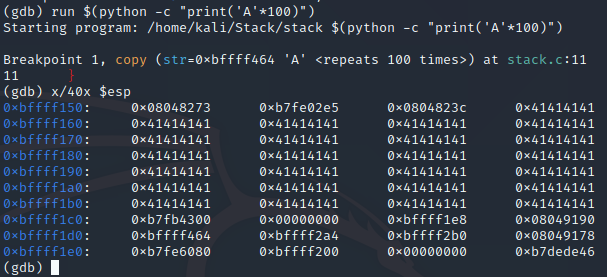
\includegraphics[scale=0.7]{images/stack_content.png}\\
  \caption{Contenido del stack}
  \label{fig:stack_content}
\end{figure}

\begin{figure}[h!]
  \centering
  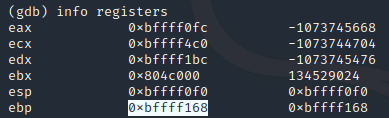
\includegraphics[scale=0.7]{images/registers.png}\\
  \caption{Los registros \$esp y \$ebp pertenecen al top y al bottom de la pila respectivamente.}
  \label{fig:registers}
\end{figure}

\begin{figure}[h!]
  \centering
  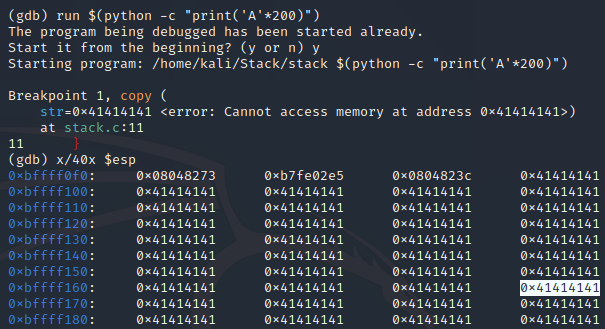
\includegraphics[scale=0.7]{images/overflow.png}\\
  \caption{Contenido del stack: La dirección de retorno (\$esp) es la seleccionada.}
  \label{fig:overflow}
\end{figure}

\begin{figure}[h!]
  \centering
  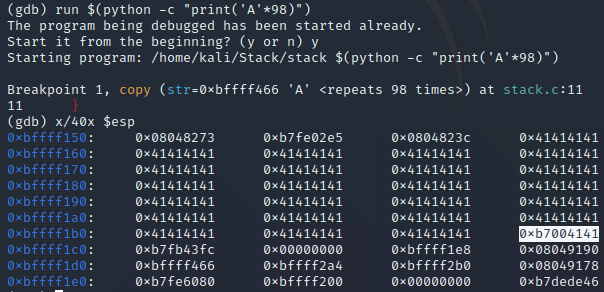
\includegraphics[scale=0.7]{images/overflow2.png}\\
  \caption{Contenido del stack: La dirección de retorno es la seleccionada. Controlamos el input exacto que tenemos que poner para controlar la dirección de retorno}
  \label{fig:overflow2}
\end{figure}

\newpage
Llegados a este punto estamos en disposición de introducir un input más elaborado que nos permita ejecutar un shellcode. Con la ayuda de este seremos capaces de inyectar en la pila el código que nos interesa ejecutar y la llamada al mismo [Ver \ref{lst:shellcode}].\\

\newpage
Existen muchos shellcodes que podemos insertar, en shell-storm.org \cite{shellstorm} encontramos una gran variedad y para reducir la cantidad de bytes a introducir en la inyección hemos seleccionado una serie de instrucciones que ejecutan el proceso \textbf{execve} en tan solo 32 bytes [Ver. \ref{lst:assembler}].\\

El método execve ejecuta un programa pasado por parámetro, haciendo que el programa que está siendo ejecutado sea substituido por el de la nueva llamada \cite{execve}; perfecto para llamar a la shell del sistema.

\begin{lstlisting}[
	language={[x86masm]Assembler}, 
	caption=Linux/x86 execve /bin/sh shellcode 23 bytes,
	label={lst:assembler}
	]
xor    %eax,%eax
push   %eax
push   $0x68732f2f
push   $0x6e69622f
mov    %esp,%ebx
push   %eax
push   %ebx
mov    %esp,%ecx
mov    $0xb,%al
int    $0x80
\end{lstlisting}

El código en hexadecimal que traduce estas instrucciones será inyectado por nuestro programa en la pila [Ver. \ref{lst:hex}].
\begin{lstlisting}[label={lst:hex}, caption=Codificación hexadecimal de las instrucciones en ensamblador]
\x31\xc0\x50\x68\x2f\x2f\x73\x68\x68\x2f\x62\x69\x6e\x89\xe3\x50\x53\x89\xe1\xb0\x0b\xcd\x80
\end{lstlisting}


El programa auxiliar de shellcode.py [Ver \ref{lst:shellcode}] nos permite introducir de manera más cómoda el shellcode necesario para ejecutar la terminal. Este programa primero escribe el carácter NOP, luego el shellcode [Ver \ref{lst:hex}], carácteres de relleno y finalmente un salto a una dirección de memoria que contenga la instrucción NOP para que esta se ignore y se ejecute la siguiente intrucción.\\

Introduciremos 64 caracteres NOP [Ver \ref{lst:nop}].

\lstinputlisting[
	language=Python,
	lastline=5,
	label={lst:nop},
	caption={[shellcode.py]{Instrucción NOP}}
]{shellcode.py}

Seguido de las instrucciones de ensamblador codificadas [Ver \ref{lst:nop}] [Ver \ref{lst:hex}].

\lstinputlisting[
	language=Python,
	firstline=6,
	lastline=10
	label={lst:nop},
	caption={[shellcode.py]{Codificación en hexadecimal de las intrucciones en ensamblador}}
]{shellcode.py}

Finalmente, crearemos un relleno con el caracter ``*'' hasta ocupar el resto de la pila y la variable eip como referencia directa a la siguiente instrucción a ejecutar ocupando la posición del instruction pointer. Su valor será el de los caracteres ``EIP'' [Ver \ref{lst:padding}].

\lstinputlisting[
	language=Python,
	firstline=12,
	lastline=14,
	label={lst:padding},
	caption={[shellcode.py]{Creación del padding y de la variable EIP}}
]{shellcode.py}

Si introducimos este programa como entrada de nuestro programa vulnerable podemos observar cómo la pila contiene la codificación del NOP (``90'' en hexadecimal), la codificación en ensamblador, unos carácteres de relleno mediante la codificación de ``*'' (``2a'' en hexadecimal) y, finalmente, en la dirección correspondiente al eip ahora tenemos insertados los bytes que corresponden a la codificación de los caracteres EIP en sentido inverso, es decir, en 0xbffff1b8 tendremos 00504945 [Fig. \ref{fig:ebp}] [Fig. \ref{fig:eip}]

\begin{figure}[h!]
  \centering
  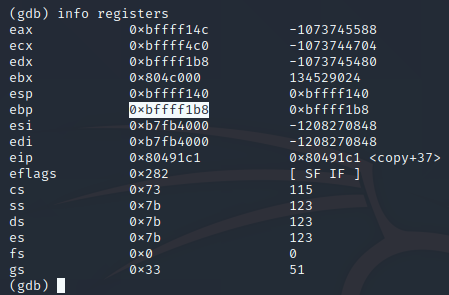
\includegraphics[scale=0.7]{images/ebp.png}\\
  \caption{Dirección de ebp (stack bottom) en esta nueva ejecución}
  \label{fig:ebp}
\end{figure}

\begin{figure}[h!]
  \centering
  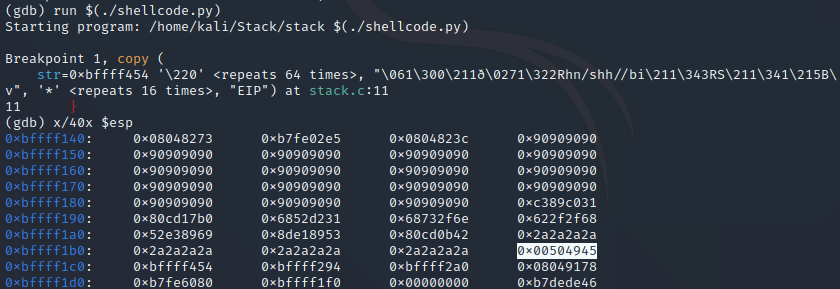
\includegraphics[scale=0.5]{images/eip.png}\\
  \caption{Contenido del stack: La dirección de retorno (\$eip) es la seleccionada correspondiente a la codificación de los caracteres EIP}
  \label{fig:eip}
\end{figure}

Ahora solo hay que cambiar el contenido de la dirección 0xbffff1b8 a una dirección que contenga un NOP y de esta forma haremos que se ejecuten las intrucciones en ensamblador, es decir, sacar una terminal. El contenido de esa dirección viene determinado por la variable ``eip'' de nuestro programa shellcode.py [Ver \ref{lst:eip2}].

\lstinputlisting[
	language=Python,
	firstline=13,
	lastline=13,
	label={lst:eip2},
	caption={[shellcode.py]{La variable EIP contiene una dirección de memoria cuyo contenido es una instrucción NOP}}
]{shellcode.py}

Cambiando el contenido de la variable eip junto a una nueva ejecución generará una pila con el contenido de la figura [Fig. \ref{fig:eip3}]. De esta forma conseguiremos ejecutar el shellcode y como resultado obtendremos una llamada a la terminal del sistema [Fig. \ref{fig:terminal}].

\newpage

\begin{figure}[h!]
  \centering
  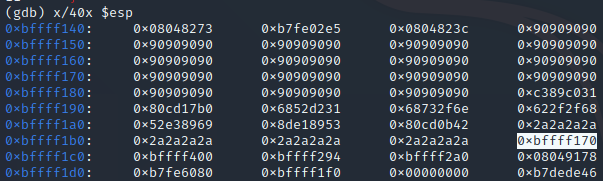
\includegraphics[scale=0.7]{images/eip3.png}\\
  \caption{Contenido del stack: La dirección de retorno (\$eip) es la seleccionada correspondiente a una con instrucción NOP}
  \label{fig:eip3}
\end{figure}

\begin{figure}[h!]
  \centering
  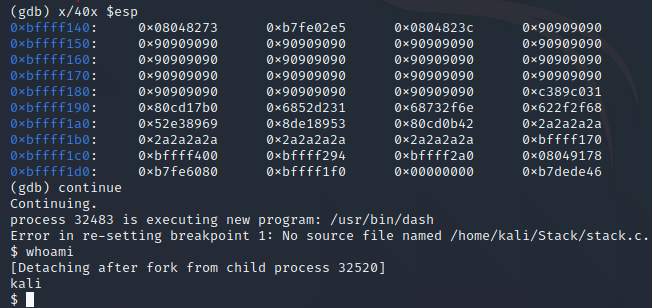
\includegraphics[scale=0.5]{images/terminal.png}\\
  \caption{Acceso a una terminal desde input con shellcode en programa vulnerable a Stack Overflow}
  \label{fig:terminal}
\end{figure}

\newpage
Para hacer un examen más exhaustivo, pasaremos a hacer el reverse engineering del shellcode proporcionado. Para esto crearemos el programa shellcode.c [Ver \ref{lst:shellcodec}], en este programa primero pondremos el código hexadecimal en una variable que luego será llamada de forma dinámica creando una función a partir del código hexadecimal.\\

Inpeccionamos el ejecutable generado por este código y ponemos un breakpoint en la llamada ret(). En el desensamblaje de este programa podemos observar una interrupción 80. Esta interrupción hace una llamada de sistema al contenido registro eax [Fig. \ref{fig:disassemble}]. 

\begin{figure}[h!]
  \centering
  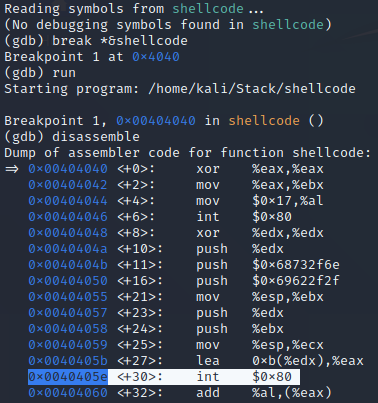
\includegraphics[scale=0.5]{images/disassemble.png}\\
  \caption{Desensamblaje del ejecutable de shellcode.c}
  \label{fig:disassemble}
\end{figure}

Volveremos a ejecutar el mismo programa con otro breakpoint, esta vez en la dirección que corresponde a la interrupción 0x0040405e. Llegados a este punto podemos analizar el contenido del registro eax: 0xb [Fig. \ref{fig:disassemble2}]. 

\begin{figure}[h!]
  \centering
  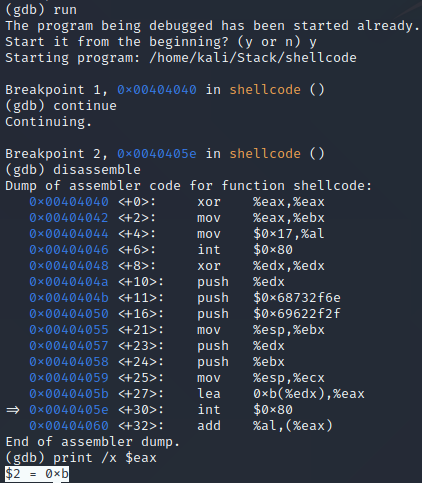
\includegraphics[scale=0.5]{images/disassemble2.png}\\
  \caption{Contenido del registro eax en la llamada del shellcode}
  \label{fig:disassemble2}
\end{figure}

``b'' en hexadecimal corresponde al 11, y este número corresponde a la instrucción definida en el fichero /usr/src/linux-headers-5.7.0-kali1-696-pae/arch/x86/include/generated/uapi/asm/unistd\_32.h.\\

En tal fichero veremos la siguiente definición \#define \_\_NR\_execve 11 con lo que podemos inferir que la interrupción está llamando al programa execve, tal como habíamos visto anteriormente [Fig. \ref{fig:execve}].

\begin{figure}[h!]
  \centering
  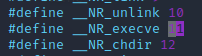
\includegraphics[scale=0.5]{images/execve.png}\\
  \caption{Definición de la función execve}
  \label{fig:execve}
\end{figure}

\newpage
\appendix
\section{stack.c}
\label{lst:stack}
\lstinputlisting[
	language=C, 
	caption={[stack.c]{Programa de stack overflow}}
]{stack.c}

\section{shellcode.py}
\label{lst:shellcode}
\lstinputlisting[
	language=Python, 
	caption={[shellcode.py]{Programa de inyección de shellcode}}
]{shellcode.py}

\section{shellcode.c}
\label{lst:shellcodec}
\lstinputlisting[
	language=C, 
	caption={[shellcode.c]{Programa para desensamblar shellcode}}
]{shellcode.c}

\newpage
\begin{thebibliography}{9}
   
\bibitem{buffer}
	\textbf{Buffer Overflow Attack}, \\
	\textit{OWASP} \\
	\url{https://owasp.org/www-community/attacks/Buffer_overflow_attack}

\bibitem{aslr}
	\textbf{3.15.1 Address Space Layout Randomization}\\
	\textit{Oracle Linux}\\
	\url{https://docs.oracle.com/cd/E37670_01/E36387/html/ol_aslr_sec.html}

\bibitem{pie}
	\textbf{Position Independent Executables (PIE)}\\
	\textit{Red Hat Customer Portal}\\
	\url{https://access.redhat.com/blogs/766093/posts/1975793}

\bibitem{strcpy}
	\textbf{STRCPY(3)}\\
	\textit{Linux manual page}\\
	\url{https://man7.org/linux/man-pages/man3/strcpy.3.html}
	
\bibitem{shellcode}
	\textbf{Shell Code For Beginners}\\
	\textit{Beenu Arora - 2007}\\
	\url{https://www.exploit-db.com/docs/english/13019-shell-code-for-beginners.pdf}

\bibitem{shellstorm}
	\textbf{Linux/x86 execve /bin/sh shellcode 23 bytes}\\
	\textit{Hamza Megahed}\\
	\url{http://shell-storm.org/shellcode/files/shellcode-827.php}
	
\bibitem{execve}
	\textbf{execve(2)}\\
	\textit{Linux manual page}\\
	\url{https://man7.org/linux/man-pages/man2/execve.2.html}
	
\bibitem{exploit}
	\textbf{Proj 3: Linux Buffer Overflow With Shellcode}\\
	\textit{samsclass.info}\\
	\url{https://samsclass.info/127/proj/p3-lbuf1.htm}
	
\bibitem{exploit}
	\textbf{BUFFER OVERFLOW 10 - Vulnerability \& Exploit Example}\\
	\textit{tenouk.com}\\
	\url{https://www.tenouk.com/Bufferoverflowc/Bufferoverflow6.html}
	
\bibitem{reverse}	
	\textbf{Linux x86 Reverse Engineering
	Shellcode Disassembling and XOR decryption}\\
	\textit{Harsh N. Daftary}
	 
\end{thebibliography}

\end{document}